\documentclass{article}

\usepackage{fancyhdr} % Required for custom headers
\usepackage{lastpage} % Required to determine the last page for the footer
\usepackage{extramarks} % Required for headers and footers
\usepackage[usenames,dvipsnames]{color} % Required for custom colors
\usepackage{graphicx} % Required to insert images
\usepackage{listings} % Required for insertion of code
\usepackage{courier} % Required for the courier font
\usepackage{lipsum} % Used for inserting dummy 'Lorem ipsum' text into the template
\usepackage{amsmath}
\usepackage{amssymb}
\usepackage{mathtools, xparse}
\usepackage{booktabs}
\usepackage{bigstrut}
\usepackage{float}
\usepackage{hyperref}
\usepackage{color}
\usepackage{algorithm}
\usepackage{caption}
\usepackage{algpseudocode}
\usepackage{multirow}


\DeclarePairedDelimiter{\norm}{\lVert}{\rVert}
\DeclarePairedDelimiter\abs{\lvert}{\rvert}%

\hypersetup{
    colorlinks   = true,    % Colours links instead of ugly boxes
    urlcolor     = red,    % Colour for external hyperlinks
    linkcolor    = red,    % Colour of internal links
    citecolor    = red      % Colour of citations
}
% Margins
\topmargin=-0.45in
\evensidemargin=0in
\oddsidemargin=0in
\textwidth=6.5in
\textheight=9.0in
\headsep=0.25in

\linespread{1.1} % Line spacing

% Set up the header and footer
\pagestyle{fancy}
\lhead{\hmwkAuthorName} % Top left header
\chead{\hmwkClass\ : \hmwkID} % Top center head
\rhead{\firstxmark} % Top right header
\lfoot{\lastxmark} % Bottom left footer
\cfoot{} % Bottom center footer
\rfoot{Page\ \thepage\ of\ \protect\pageref*{LastPage}} % Bottom right footer
\renewcommand\headrulewidth{0.4pt} % Size of the header rule
\renewcommand\footrulewidth{0.4pt} % Size of the footer rule

\setlength\parindent{0pt} % Removes all indentation from paragraphs

%----------------------------------------------------------------------------------------
%	CODE INCLUSION CONFIGURATION
%----------------------------------------------------------------------------------------

\definecolor{MyDarkGreen}{rgb}{0.0,0.4,0.0} % This is the color used for comments
\lstloadlanguages{Perl} % Load Perl syntax for listings, for a list of other languages supported see: ftp://ftp.tex.ac.uk/tex-archive/macros/latex/contrib/listings/listings.pdf
\lstset{language=Perl, % Use Perl in this example
    frame=single, % Single frame around code
    basicstyle=\small\ttfamily, % Use small true type font
    keywordstyle=[1]\color{Blue}\bf, % Perl functions bold and blue
    keywordstyle=[2]\color{Purple}, % Perl function arguments purple
    keywordstyle=[3]\color{Blue}\underbar, % Custom functions underlined and blue
    identifierstyle=, % Nothing special about identifiers                                         
    commentstyle=\usefont{T1}{pcr}{m}{sl}\color{MyDarkGreen}\small, % Comments small dark green courier font
    stringstyle=\color{Purple}, % Strings are purple
    showstringspaces=false, % Don't put marks in string spaces
    tabsize=5, % 5 spaces per tab
    %
    % Put standard Perl functions not included in the default language here
    morekeywords={rand},
    %
    % Put Perl function parameters here
    morekeywords=[2]{on, off, interp},
    %
    % Put user defined functions here
    morekeywords=[3]{test},
    %
    morecomment=[l][\color{Blue}]{...}, % Line continuation (...) like blue comment
    numbers=left, % Line numbers on left
    firstnumber=1, % Line numbers start with line 1
    numberstyle=\tiny\color{Blue}, % Line numbers are blue and small
    stepnumber=5 % Line numbers go in steps of 5
}

% Creates a new command to include a perl script, the first parameter is the filename of the script (without .pl), the second parameter is the caption
\newcommand{\perlscript}[2]{
    \begin{itemize}
        \item[]\lstinputlisting[caption=#2,label=#1]{#1.py}
    \end{itemize}
}
\newcommand{\cppscript}[1]{
    \begin{itemize}
        \item[]\lstinputlisting[]{#1}
    \end{itemize}
}

%----------------------------------------------------------------------------------------
%	DOCUMENT STRUCTURE COMMANDS
%	Skip this unless you know what you're doing
%----------------------------------------------------------------------------------------

% Header and footer for when a page split occurs within a problem environment
\newcommand{\enterProblemHeader}[1]{
    \nobreak\extramarks{#1}{#1 continued on next page\ldots}\nobreak
    \nobreak\extramarks{#1 (continued)}{#1 continued on next page\ldots}\nobreak
}

% Header and footer for when a page split occurs between problem environments
\newcommand{\exitProblemHeader}[1]{
    \nobreak\extramarks{#1 (continued)}{#1 continued on next page\ldots}\nobreak
    \nobreak\extramarks{#1}{}\nobreak
}

%\setcounter{secnumdepth}{0} % Removes default section numbers
\newcounter{homeworkProblemCounter} % Creates a counter to keep track of the number of problems

\newcommand{\homeworkProblemName}{}
\newenvironment{homeworkProblem}[1][Problem \arabic{homeworkProblemCounter}]{ % Makes a new environment called homeworkProblem which takes 1 argument (custom name) but the default is "Problem #"
    \stepcounter{homeworkProblemCounter} % Increase counter for number of problems
    \renewcommand{\homeworkProblemName}{#1} % Assign \homeworkProblemName the name of the problem
    \section{\homeworkProblemName} % Make a section in the document with the custom problem count
    \enterProblemHeader{\homeworkProblemName} % Header and footer within the environment
    }{
    \exitProblemHeader{\homeworkProblemName} % Header and footer after the environment
}

\newcommand{\problemAnswer}[1]{ % Defines the problem answer command with the content as the only argument
\noindent\framebox[\columnwidth][c]{\begin{minipage}{0.98\columnwidth}#1\end{minipage}} % Makes the box around the problem answer and puts the content inside
}

\newcommand{\homeworkSectionName}{}
\newenvironment{homeworkSection}[1]{ % New environment for sections within homework problems, takes 1 argument - the name of the section
    \renewcommand{\homeworkSectionName}{#1} % Assign \homeworkSectionName to the name of the section from the environment argument
    \subsection{\homeworkSectionName} % Make a subsection with the custom name of the subsection
    \enterProblemHeader{\homeworkProblemName\ [\homeworkSectionName]} % Header and footer within the environment
    }{
    \enterProblemHeader{\homeworkProblemName} % Header and footer after the environment
}

%----------------------------------------------------------------------------------------
%	NAME AND CLASS SECTION
%----------------------------------------------------------------------------------------

\newcommand{\hmwkID}{homework 08} % Assignment title
\newcommand{\hmwkTitle}{Polynomial Interpolations}
\newcommand{\hmwkDueDate}{Tuesday,\ April\ 25,\ 2017} % Due date
\newcommand{\hmwkClass}{Numerical Analysis} % Course/class
\newcommand{\hmwkClassTime}{10:30am} % Class/lecture time
\newcommand{\hmwkClassInstructor}{Jones} % Teacher/lecturer
\newcommand{\hmwkAuthorName}{102061149 Fu-En Wang} % Your name

%----------------------------------------------------------------------------------------
%	TITLE PAGE
%----------------------------------------------------------------------------------------

\title{
    \vspace{2in}
    \textmd{\textbf{\hmwkClass}}\\
    \textmd{\textbf{\hmwkID: \hmwkTitle}} \\
    \normalsize\vspace{0.1in}\small{Due\ on\ \hmwkDueDate}\\
    \vspace{3in}
}

\author{\textbf{\hmwkAuthorName}}
\date{} % Insert date here if you want it to appear below your name

%----------------------------------------------------------------------------------------

\begin{document}
\maketitle
\newpage

\section{Introduction}
When recording experiment data, we usually have no time to record densely. However, to get the value of certain
range we skip, we need to use interpolation to find it out. In this homework, we will use \textbf{Lagrange Interpolation} to
recover the waveform and compare it with the groundtruth data.
\subsection{Lagrange Interpolation}
Give a set of support points $\{(x_i, y_i), 0 \leq i \leq n\}$, then
\begin{align}
    F(x) = \sum_{i=0}^{n}y_i\prod_{k=0,k \neq i}^{n}\frac{x-x_k}{x_i-x_k}
\end{align}
where $F(x)$ is interpolated value of location $x$.

\section{Implementation}
\begin{algorithm}[H]
    \caption{\textbf{Non-recursive Nevile's Algorithm}}
    \label{algo:nevile}
    \begin{algorithmic}
        \State XS, YS is support data, x is location to interpolate.
        \State NS = YS
        \For{each k $\in$ \{1,...., n-1\}}
            \For{each j $\in$ \{0,..., n-k-1\}}
                \State NS[j] = ((x-XS[j])*NS[j+1]-(x-XS[k+j])*NS[j]) / (XS[j+k]-XS[j])
            \EndFor
        \EndFor
        \State return NS[0]
    \end{algorithmic}
\end{algorithm}

\subsection{Complexity}
\label{sec:complexity}
From Algorithm \ref{algo:nevile}, the double for-loop make the whole process a {\boldmath$O(n^2)$} problem.

\section{Discussion}
In this section, we will discussion the folowing topics:
\begin{enumerate}
    \item Experiment result of \textbf{f3.dat, f5,dat, f7,dat, f13.dat, f21.dat}
    \item Maximum error against \textbf{f301.dat}, which is our groundtruth
    \item Maximum error(x=550 to 700) against \textbf{f301.dat}, which is our groundtruth
\end{enumerate}
\newpage
\subsection{Maximum Error}
Table \ref{tab:error} shows the result of all dat.
% Table generated by Excel2LaTeX from sheet '工作表1'
\begin{table}[H]
  \centering
    \begin{tabular}{|c|c|c|c|c|c|}
    \hline
        & f3  & f5  & f7  & f13 & f21 \bigstrut\\
    \hline
    Max Error(all) & 372.866858 & 248.340631 & 379.107286 & 1283.4489 & 16728.5648 \bigstrut\\
    \hline
    Max Error(550 to 700) & 372.866858 & 233.364371 & 148.890794 & 39.618945 & 17.803983 \bigstrut\\
    \hline
    \end{tabular}%
  \caption{Max error of all dat}
  \label{tab:error}%
\end{table}%
In Table \ref{tab:error}, Max Error(550 to 700) decreases when using more support points. However, Max Error(all) increases
when using more support points. Because the range of interpolation is from 475 to 775, so the maximum error should occut at the
475 to 549 or 701 to 775.

\subsection{Experiment Result}
In this section we will plot the interpolated data along with the original data to find out some problems of 
\textbf{Lagrange Interpolation}. The following figures show the experiment result of f3.dat to f21.dat.
\begin{figure}[H]
    \centering
    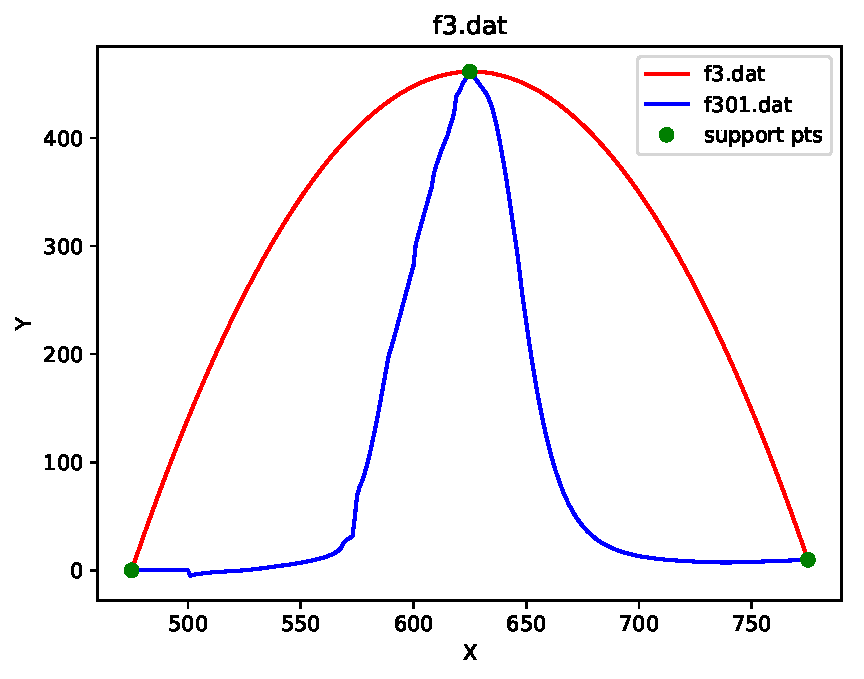
\includegraphics[width=0.7\textwidth]{src/f3.pdf}
    \caption{Result of f3.dat}
    \label{fig:f3}
\end{figure}
The number of support points in Figure \ref{fig:f3} is 3, so the interpolated data will be a second order polynomial and has a
huge error with groundtruth.

\begin{figure}[H]
    \centering
    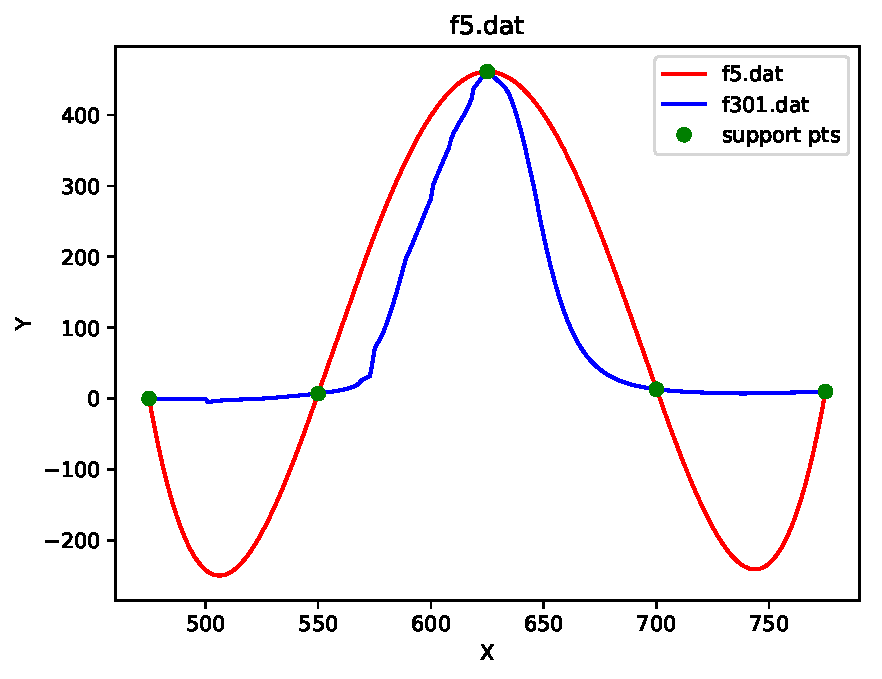
\includegraphics[width=0.7\textwidth]{src/f5.pdf}
    \caption{Result of f5.dat}
    \label{fig:f5}
\end{figure}
\begin{figure}[H]
    \centering
    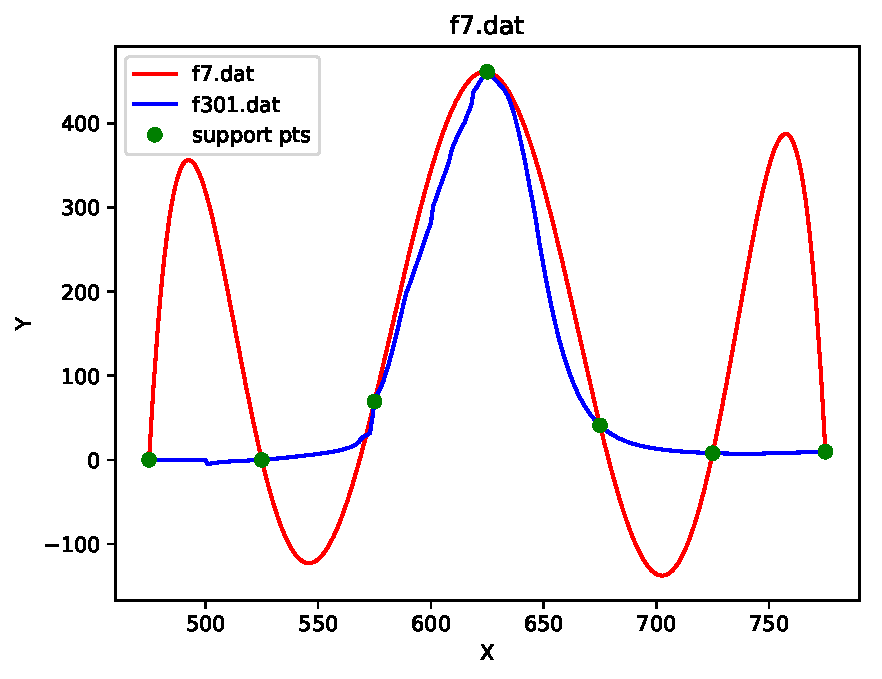
\includegraphics[width=0.7\textwidth]{src/f7.pdf}
    \caption{Result of f7.dat}
    \label{fig:f7}
\end{figure}
In Figure \ref{fig:f5} and \ref{fig:f7}, the order of polynomial become 4 and 6 and our interpolated data match the support points.
But the number of support points seems still not enough to recover the origin data.
\begin{figure}[H]
    \centering
    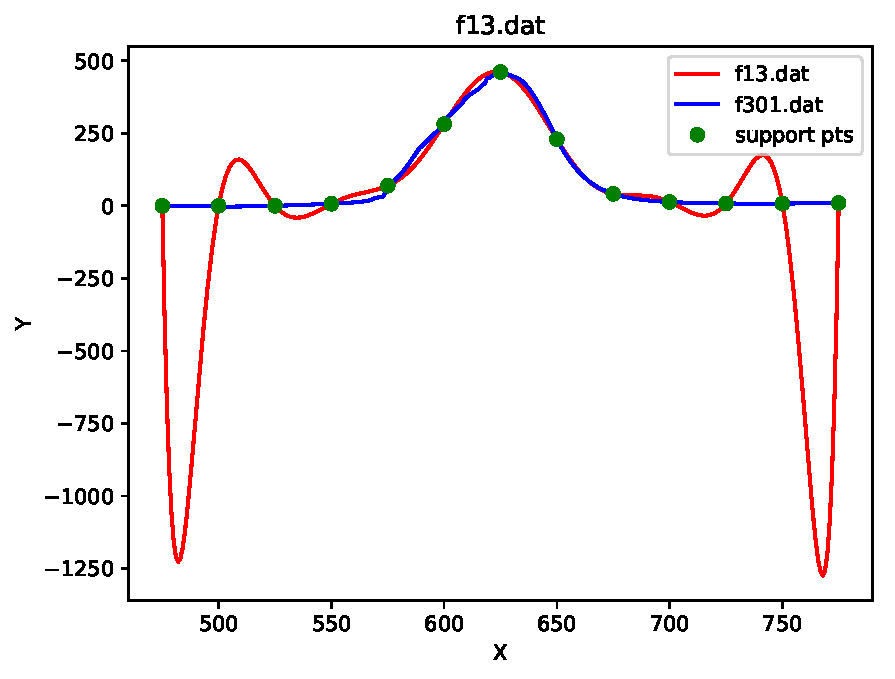
\includegraphics[width=0.7\textwidth]{src/f13.pdf}
    \caption{Result of f13.dat}
    \label{fig:f13}
\end{figure}
\begin{figure}[H]
    \centering
    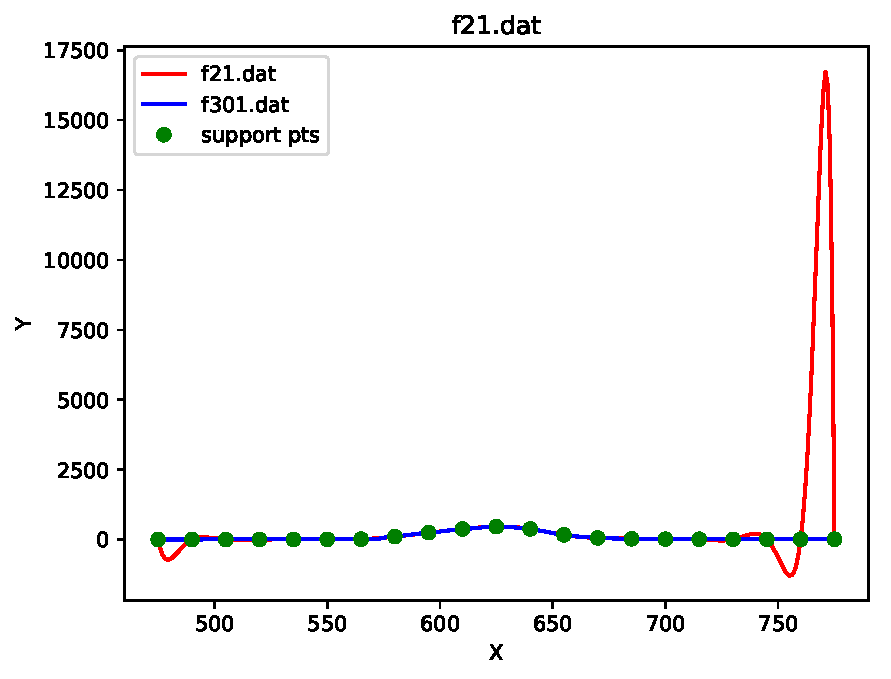
\includegraphics[width=0.7\textwidth]{src/f21.pdf}
    \caption{Result of f21.dat}
    \label{fig:f21}
\end{figure}
In Figure \ref{fig:f13} and \ref{fig:f21}, the mid part of interpolated value is very close to the origin one, but the left and 
right side  have a great error. Because when number of support points is large, the interpolated polynomial will have a large order 
and $x^n$ will cause a huge error. As a result, \textbf{round-off error} will be very large at the
two side of interpolation. So when we use Lagrange Interpolation, we have to prevent ourself from getting value at
the neighbor of two side. In addition, we should also prevent extrapolation, because Largrange also has large error at location 
out of support point range.

\section{Conclusion}
From the result in Figure \ref{fig:f13} and \ref{fig:f21}, Lagrange Interpolation can be pretty accurate at the mid part of
data but has huge error at the two side. So if we need to get data at the two side, we should prevent ourself from using
this algorithm.

\end{document}













